\documentclass{article}
\usepackage[utf8]{inputenc}
\usepackage{geometry}
\geometry{a4paper, margin=1in}
\usepackage{graphicx}
\usepackage{hyperref}
\usepackage{fancyhdr}

\setlength{\headheight}{15pt}
\pagestyle{fancy}
\fancyhf{}
\rhead{Computer Workshop Course}
\lhead{Final Assignment}
\begin{document}

\begin{titlepage}
\title{
\textbf{In the Name of God the Beneficent}\par
    \vspace{2in}

\textbf{Final Assignment:}\par

\textbf{Integration of Tools and Practices}\par
    \vspace{2in}
}
\author{Seyed Ahmad Mousavi}

\date{\today}
\maketitle
\thispagestyle{empty}
\end{titlepage}
%new page
\newpage

\tableofcontents

\fancyfoot[R]{page \thepage}
\fancyfoot[C]{}
%new page
\newpage
\section{Git and GitHub}
\subsection{Repository Initialization and Commits}
\begin{enumerate}
    \item {At first i made a directory in my device and then i made .github then workflows in that and copy past main.yml wich was in \url{https://github.com/MiliAxe/CW1402Final/tree/master} .}
    \item {I made a new repsitory in my github .}
    \item {I connect my diroctory to my repo with repostory's SSH .}
    \item {After thease all with making tags and push commits on tags ,\textbf{Git Actions} make a release by tags and give us a document in releases .}
\end{enumerate}
\subsection{GitHub Actions for LaTeX Compilation}
\begin{enumerate}
    \item {According to what was said in the Guide doc i copy main.yml to my workflows .}
    \item {What is on workflows runs by \textbf{Git Actions} .}
    \item {The main.yml basically creates generated PDF file from provided Latex file, it can be set in workflow file as given . this workflow runs on tagged commits which has a tag with *.*.* pattern .}
    \item {Some jobs of this orkflow is :}
    	\begin{itemize}
    		\item{ runing on tagged commits which has a tag with *.*.* }
    		\item{Create Release }
    		\item{ and Upload Release .}
    	\end{itemize}
\end{enumerate}
\section{Exploration Tasks}
\subsection{Vim Advanced Features}
\begin{enumerate}
    \item{To replace text, enter Normal mode and type (:\%s/old/new/g) , where old is the text that you want to replace, and new is the replacement text.}
    \item{To automatically indent new lines based on the indentation of the previous line, type (:set autoindent) .}
    \item{To exit the text editor without saving any changes, press (:q!) .}
\end{enumerate}
\subsection{Memory profiling}
\subsubsection{Memory Leak}
In conclusion, memory leaks can occur when we allocate memory on the heap but forget to release it or free it. Due to memory leaks, we may experience performance degradation and system becomes unstable. Memory leaks cause more damage for long-running programs like servers .

\subsubsection{Memory profilers}
In conclusion, memory leaks can occur when we allocate memory on the heap but forget to release it or free it. Due to memory leaks, we may experience performance degradation and system becomes unstable. Memory leaks cause more damage for long-running programs like servers .
\newpage
\subsection{GNU/Linux Bash Scripting}
\subsubsection{fzf}
\begin{enumerate}
    \item{A fuzzy search searches for text that matches a term closely instead of exactly. Fuzzy searches help you find relevant results even when the search terms are misspelled .}
    \item{If we write \texttt{ls | fzf} in terminal we will see a list of every thing is near to what we are typing .}
\end{enumerate}
\subsubsection{Using fzf to find your favorite PDF}
\begin{enumerate}
    \item{fd -e pdf }
    \item{\texttt{fd -e pdf | fzf}}
\end{enumerate}
\subsubsection{Opening the file using Zathura}
\begin{itemize}
    \item{\texttt{zathura \$(fd -e pdf | fzf)}}
\end{itemize}
\section{Git and Foss}
\subsection{README.md}
\begin{itemize}
    \item{done}
\end{itemize}
\subsection{Issues}
\begin{figure}[h]
\centerline{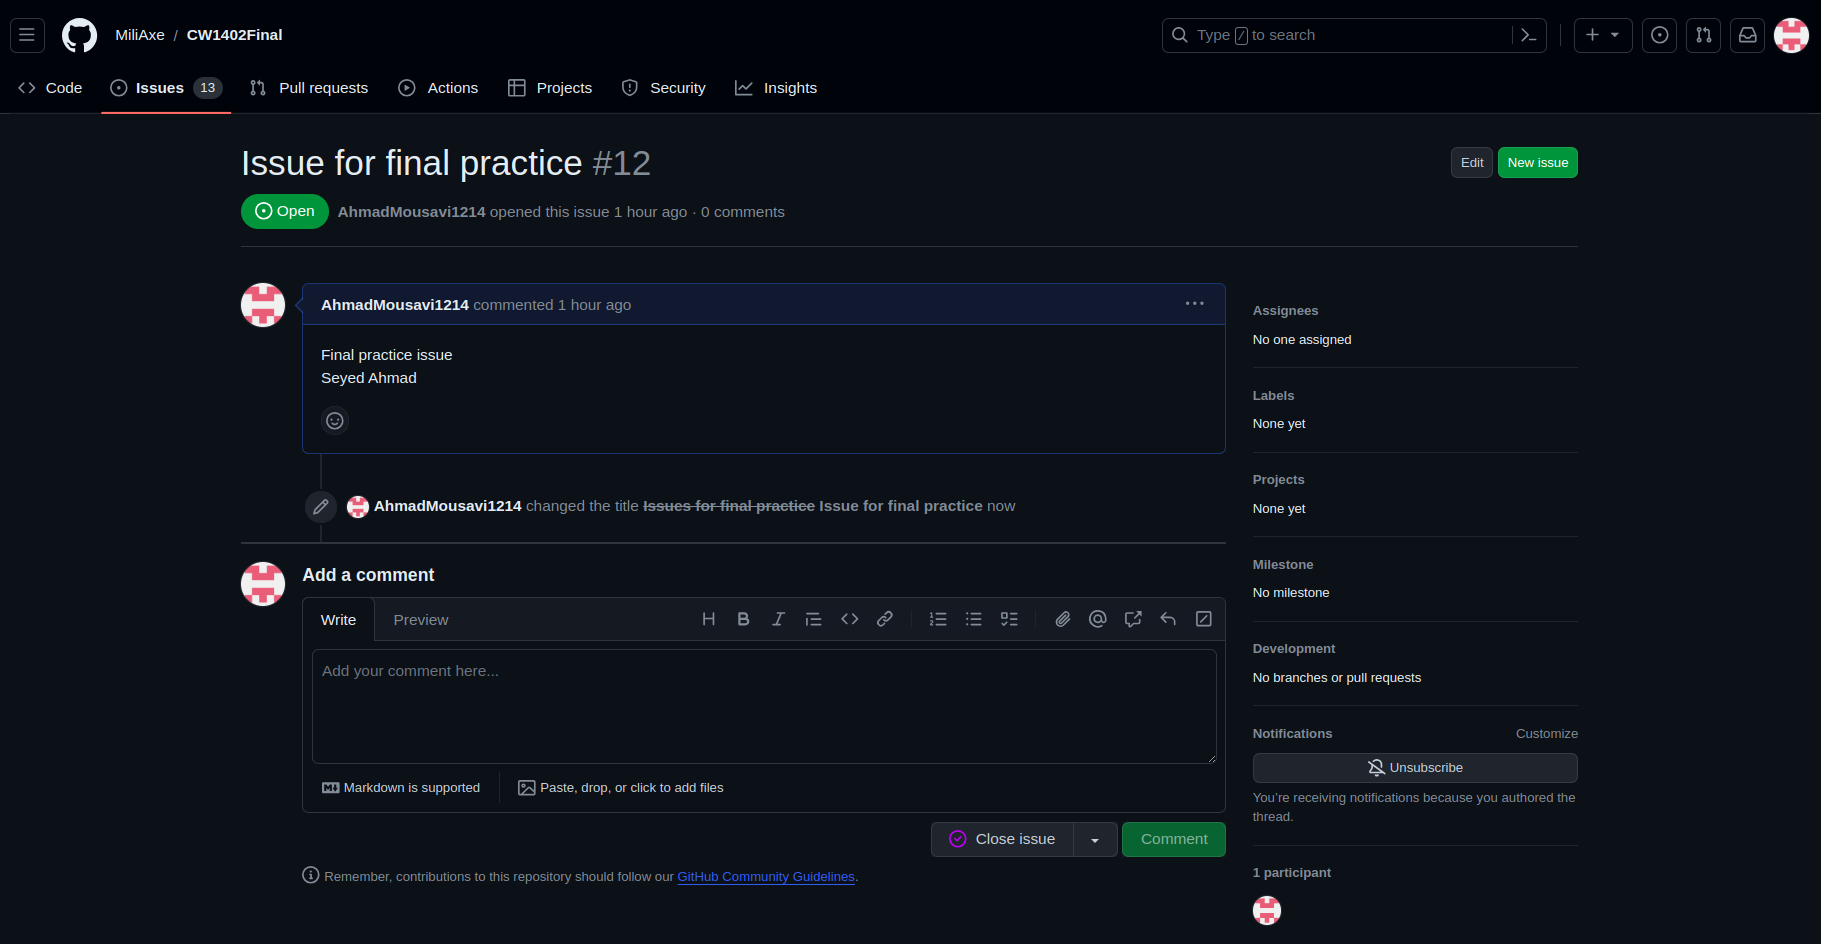
\includegraphics[width = 0.8\textwidth]{issue.png}}
\caption{My Issue}
\label{fig}
\end{figure}
\end{document}
